\chapter{Analisi del protocollo RLN}
\chaptermark{Analisi del protocollo RLN}
\label{chap:rln-protocol}

Nel presente capitolo, tratteremo la discussione del protocollo RLN (Rate Limiting Nullifier), che consente la
costruzione di regole di rate-limiting anti DoS e spam in ambiente anonimo utilizzando la tecnologia zk-SANRK. La prima proposta del protocollo è stata
sviluppata da Barry WhiteHat, un ricercatore attivo nel campo della blockchain e delle applicazioni Zero Knowledge, nel
seguente post: "Semaphore RLN, rate-limiting nullifier for spam prevention in anonymous p2p setting" \cite{semaphore-rln}. Attualmente, RLN
fa parte di (PSE) Privacy \& Scaling Explorations \cite{pse}, un team multidisciplinare sostenuto dalla Fondazione Ethereum, che
esplora nuove tecnologie Zero Knowledge e altre primitive crittografiche. Alcuni progetti di rilievo includono zk-kit,
Interep e Semaphore. RLN è ancora un protocollo poco conosciuto, e non esistono ancora grosse implementazioni al di
fuori del contesto di ricerca. Il progetto in stato più avanzato è relativo a un lavoro portato avanti da Vac che sta
lavorando sull'implementazione del protocollo all'interno di Waku v2, la seconda versione di un protocollo di
comunicazione peer-to-peer privacy-preserving in ambiente decentralizzato.

Nelle prossime sezioni, verranno dettagliate le fasi del protocollo e le tecnologie utilizzate. Tuttavia, prima di
addentrarci, potrebbe essere utile fornire una descrizione generale e concisa del protocollo per comprendere meglio dove
e perché vengono impiegate le tecnologie che andremo a esaminare. Il protocollo RLN è suddiviso in tre fasi. Descriveremo brevemente le prime due fasi, in quanto la terza diventa ovvia una volta compreso il funzionamento delle prime due.

\textbf{Regitrazione}: Questa fase consente agli utenti di registrarsi al servizio che utilizza il protocollo RLN. In
particolare, agli utenti viene richiesto di generare una chiave privata che rappresenta il loro segreto. Le strategie
per la generazione della chiave possono variare a seconda del contesto applicativo e possono essere correlate alla
presenza o meno di una stake. Una volta ottenuta la chiave privata, a questa viene applicata una funzione di hash per
generare un "identity commitment", ovvero un dato che può essere reso pubblico in quanto non consente di ricostruire la
chiave privata, ma che ne garantisce l'identificazione univoca. Durante questa fase, l'identity commitment generato
viene inviato al servizio, che lo inserisce in una particolare struttura dati chiamata albero di Merkle. In questo
albero, il sistema salva e mantiene tutti gli identity commitment degli utenti registrati. La registrazione rappresenta
una fase cruciale del protocollo, in quanto solo dopo di essa gli utenti saranno in grado di interagire con il sistema,
generando delle Zero Knowledge proof che attestino la loro appartenenza al servizio questa prova è anche chiamata "proof
of membership". Al fine di limitare gli attacchi DoS o Sybil, la fase di registrazione sarà molto più efficace se
sottoposta al rispetto di determinate specifiche di difficile riproducibilità da parte degli utenti. Per questo, in
alcuni casi, è possibile legare la chiave privata a una stake.

\textbf{Interazione}: Questa fase rappresenta sia quella che consente l'interazione tra gli utenti registrati e il sistema, sia quella che implementa la regola di rate limiting. La chiave privata dell'utente, prima che interagisca con il sistema, viene suddivisa in $n$ parti in modo che ad ogni interazione il sistema riveli all'utente solo una porzione della chiave. Il sistema non sarà in grado di ricostruire la chiave privata dell'utente dalle singole porzioni, a meno che queste non raggiungano un numero $k$ stabilito dalla regola di rate limiting. In caso contrario, se il sistema dispone di k parti della chiave, è in grado di ricavare l'identità dell'utente. Questo processo è attuabile grazie ad un algoritmo basato sull'interpolazione di Lagrange, chiamato Shamir Secret Sharing (SSS).
\section{Strumenti}
\subsection{Alberi di Merkle}

Gli alberi di Merkle sono una particolare struttura ad albero che sfrutta le proprietà delle funzioni di hash al fine di
ottimizzare le operazioni di ricerca e identificazione delle modifiche all'interno della collezione. La struttura degli
alberi di Merkle è composta dalle foglie, che rappresentano i dati a cui è stata applicata una funzione di
hash e dai nodi, che sono ottenuti uno dopo l'altro applicando la funzione hash ai loro figli, fino a raggiungere
la radice. Negli alberi di Merkle la radice è una funzione hash che rappresenta univocamente la struttura. Per capire
meglio il concetto immaginiamo di avere un struttura ad albero binaria, e inseriamo all'interno della struttura gli
elementi 1,2,3,4 e 5 a cui applichiamo una funzione hash, a questo punto otterremo la seguente struttura:
\begin{figure}[H]
    \centering
    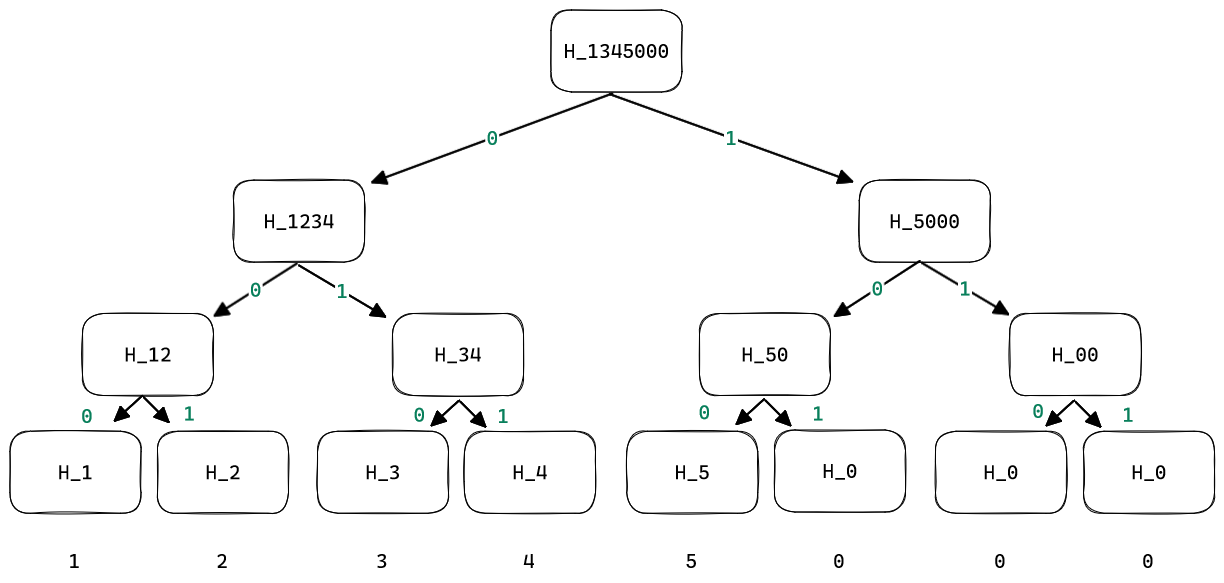
\includegraphics[width=13cm]{./chapters/2.rln-protocol/images/1.merkle_tree.png}
    \label{fig:merkle_tree}
    \captionsetup{justification=centering}
    \caption{Struttura albero di Merkle binario}
\end{figure}
Possiamo notare che la radice degli alberi di Merkle possiede la proprietà di essere una sorta di impronta digitale
della struttura, in quanto qualsiasi modifica ai dati comporterebbe un cambiamento a cascata dei nodi fino alla radice
stessa. Questa proprietà costituisce un vantaggio significativo in termini di efficienza. Infatti, consente una verifica
rapida delle modifiche apportate alla struttura, rendendo gli alberi di Merkle estremamente utili nei campi
decentralizzati e nei file system condivisi, dove l'individuazione efficiente dei cambiamenti con poche informazioni è
cruciale. Un'altra proprietà altamente utile degli alberi di Merkle è la loro capacità di verificare l'appartenenza di
un elemento alla struttura in modo efficiente e senza la necessità di conoscere l'elemento in chiaro. Nell'esempio
precedente, se si desidera verificare che l'elemento 4 appartenga alla struttura, è sufficiente utilizzare gli elementi
H\_3, H\_12 e H\_5000 e il valore H\_4, che non rivela alcuna informazione su l'elemento. Una volta ottenuta la radice
basterà confrontarla con la radice corretta per convincersi della presenza dell'elemento o meno nella struttura.
\begin{figure}[H]
    \centering
    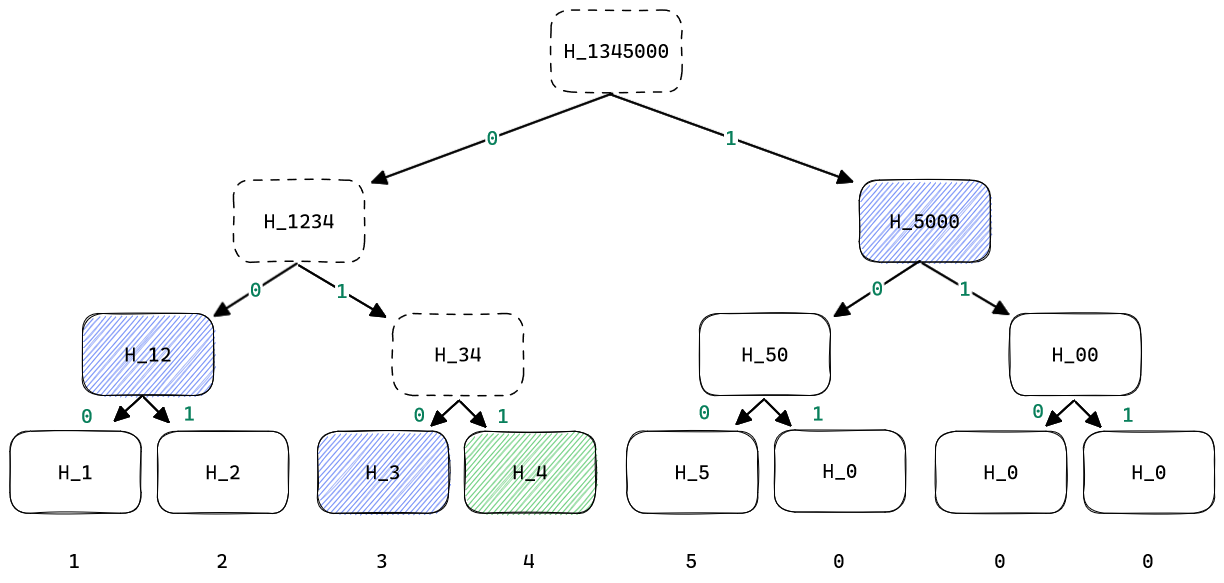
\includegraphics[width=14cm]{./chapters/2.rln-protocol/images/2.merkle_proof.png}
    \label{fig:merkle_proof}
    \captionsetup{justification=centering}
    \caption{Merkle proof}
\end{figure}
Questo processo viene chiamato "Merkle proof" o più in generale "proof of membership". Tale processo rappresenta
l'approccio che adotteremo per dimostrare la capacità di un utente già registrato e non rimosso di interagire con il
sistema nella fase di Interazione del protocollo RLN.

\subsection{Nuove funzioni di hash}
Indubbiamente, una delle tecniche più utilizzate in crittografia sono le funzioni di hash. Anche la tecnologia zk-SNARK
non può fare a meno di esse. Infatti, come abbiamo già visto in molte situazioni, l'utilizzo di metodi di hashing è
stato necessario per ridurre le dimensioni delle informazioni e per nasconderle. Tuttavia, quando si utilizzano le
tradizionali funzioni di hash come la versione Sha-256 nel campo delle Zero Knowledge proof, si verifica un problema.
Queste funzioni non sono state concepite per lavorare in domini di campi finiti e, pertanto, sfruttano metodologie come
la ripetizione di operazioni bit-wise, che tendono se trasformate con R1CS ad aumentare considerevolmente la dimensione
dei vincoli del circuito. Questo aumenta notevolmente il tempo e la dimensione richiesti
per generare le prove. Negli ultimi anni, per superare il problema descritto, sono state utilizzate nuove versioni di
funzioni hash come Pedersen, Rescue-$x^5$ e Poseidon. Queste funzioni sono state progettate specificamente per lavorare nei
campi finiti e con l'obiettivo di ridurre al minimo i tempi di generazione e i vincoli necessari per costruire le prove.
Tra queste funzioni, la funzione Poseidon è quella che ha ottenuto i risultati migliori e che verrà utilizzata nella
costruzione del circuito per il protocollo RLN. Di seguito vengono mostrate delle tabelle contenenti un confronto delle
prestazioni tra le più note funzione di hash per le tecnologie Zero Knowledge e la funzione Sha-256, tabelle tratte da
"POSEIDON: A New hash Function for Zero-Knowledge Proof Systems" \cite{cryptoeprint:2019-458}. Nelle tabelle sottostanti
possiamo notare che ci sono diverse configurazioni della funzione Poseidon. Infatti, una grande differenza tra le
funzioni tradizionali e Poseidon è la possibilità di scegliere il numero di iterazioni e la dimensione del campo finito
su cui lavorare, in modo da selezionare la versione più performante a seconda del caso.\\
\begin{figure}[H]
    \centering
    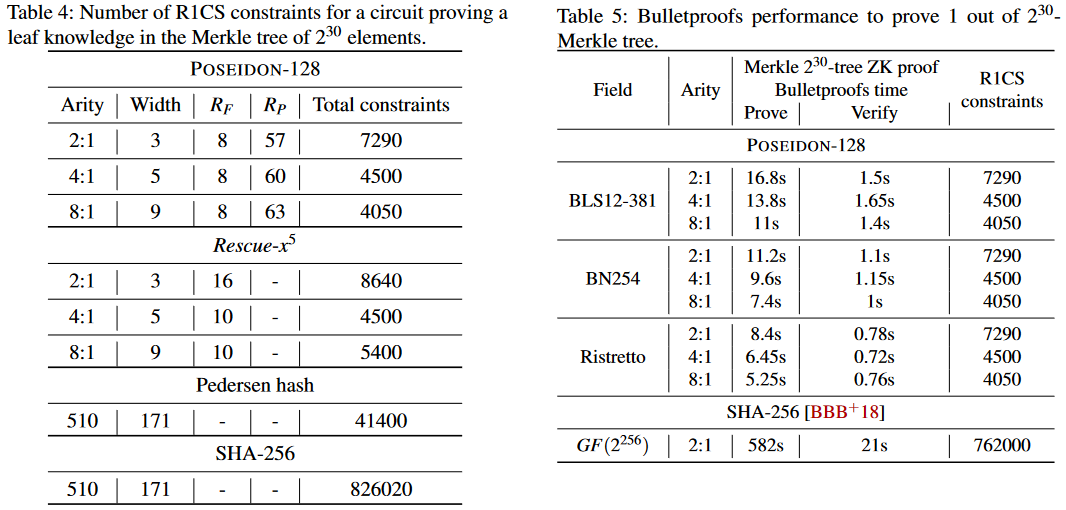
\includegraphics[width=14cm]{./chapters/2.rln-protocol/images/3.poseidon_comparison.png}
    \label{fig:poseidon_comparison}
    \captionsetup{justification=centering}
    \caption{Confronto algoritmi di hash, tratto da \cite{cryptoeprint:2019-458}}
\end{figure}

\subsection{Nullifier}
I "nullifier" in crittografia sono dei valori utilizzati per confermare o annullare operazioni. Nelle applicazioni che garantiscono
l'anonimato, questi valori vengono spesso utilizzati per evitare il problema del "double-signaling", ovvero impedire che
un utente utilizzi o esegua un'operazione che dovrebbe essere unica per ogni utente più di una volta. Questo problema
può verificarsi perché, in assenza di un collegamento tra i dati e le identità degli utenti, non è possibile verificare
se un utente ha già effettuato o completato una determinata operazione. Ad esempio, in un'applicazione elettorale è
importante impedire che un singolo elettore, voti più di una volta, mentre nel campo delle criptovalute è fondamentale evitare che la
stessa moneta, venga spesa più volte. Il problema si risolve utilizzando i nullifier ovvero valori univoci legati
all'operazione che rimangono privati fino al momento dell'effettuazione dell'operazione e una volta attuata vengono
resi pubblici, e salvati in modo da poterli consultare successivamente.
\begin{figure}[H]
    \centering
    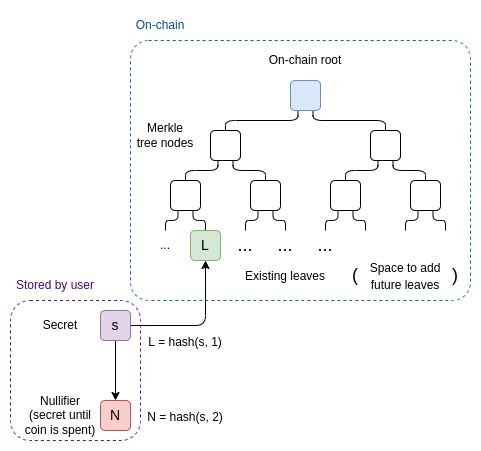
\includegraphics[width=10cm]{./chapters/2.rln-protocol/images/4.nullifier.png}
    \label{fig:nullifier}
    \captionsetup{justification=centering}
    \caption{Esempio Nullifier, tratta da \cite{some-ways-to-use-zk-snarks-for-privacy}}
\end{figure}
Dalla descrizione fornita potrebbe subito venire in mente il concetto di "rate-limiting" e si potrebbe pensate di
utilizzare i nullifier per attuare questa procedura in modo anonimo. In effetti, è possibile limitare gli
utenti utilizzando questa metodologia, però non si potrà rivelare l'identità dell'utente malintenzionato che, in questo
modo, potrebbe riprovare indisturbato ad attaccare il sistema.

Dopo aver visto le tecnologie utilizzate nel protocollo RLN, è possibile procedere con la descrizione delle sue fasi.
\begin{figure}[H]
    \centering
    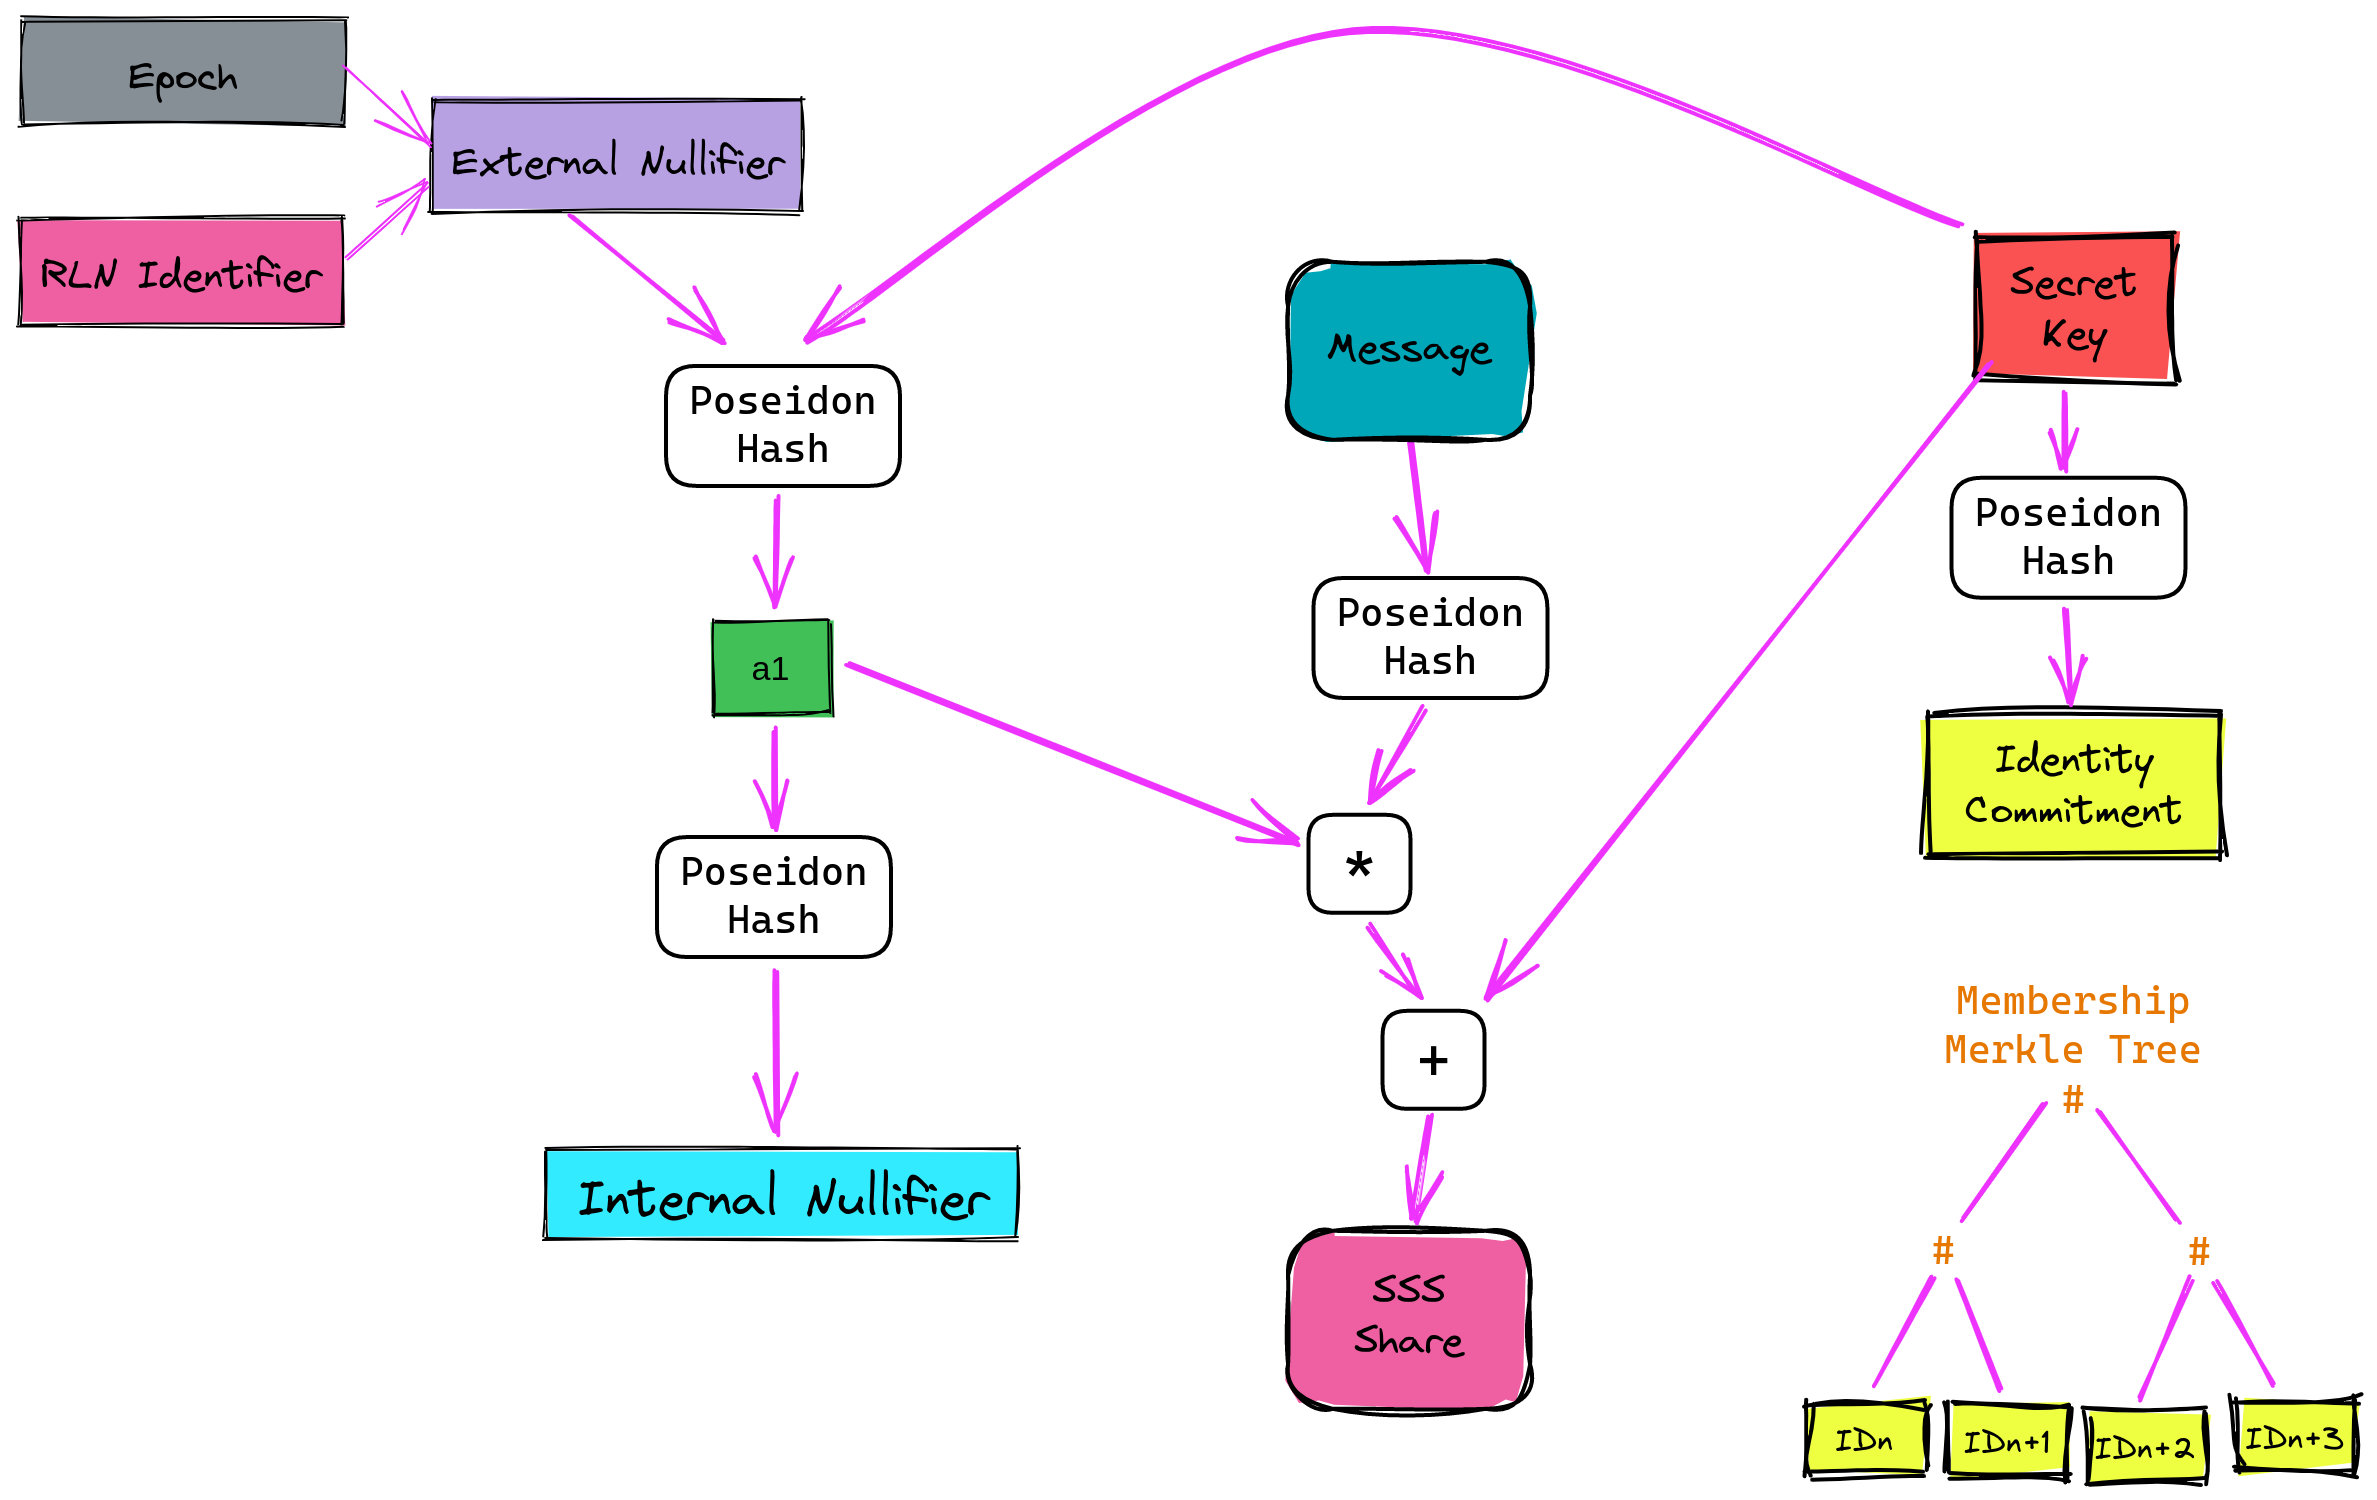
\includegraphics[width=13cm]{./chapters/2.rln-protocol/images/5.rln_flow.png}
    \label{fig:rln_flow}
    \captionsetup{justification=centering}
    \caption{Diagramma funzionametno RLN, tratto da \cite{rln_doc}}
\end{figure}

\section{Registrazione}
La registrazione consiste nella prima fase del protocollo RLN, in questa fase gli utenti, previa la generazione di una chiave privata e ricavando da questa un "identity commitment" utilizzando la funzione hash Poseidon. Per semplificare la spiegazione da qui in poi, utilizzeremo il simbolo $a_0$ per indicare la chiave privata.
$$identityCommitment = Poseidon(a_0)$$
in alcuni casi potremmo avere la necessità di elaborare maggiormente la creazione dell'identity commitment per aumentare il livello di sicurezza o associare all'identity commitment anche una stake. Una volta generato l'identity commitment l'utente viene inserito all'interno del albero di Merkel del sistema. A questo punto l'utente sarà in grado di generare dell "proof of membership" e quindi di interrogare il sisteam. Per evitare attacchi di tipo Sybil, è posibile implementare dell'tecniche che vincolino l'inserimento dell'utente nell albero al rispetto di alcuni vincoli, come posseso identità digitali o di un profilo social accreditato o ancora un portafolgio di criptovalute.

Tra i progetti del gruppo PSE troviamo anche un progetto chiamato Interep, il cui scopo è essenzialemtene estrapolare la reputazione di un utente e inserire un identity commitment a lui associato all'inetrno di alcuni gruppi di reputazione. Questi gruppi (alberi di Merkel) sono divisi in base al grado di reputazione degli utenti. Attualemente il progetto Iterep permette di estrapolare la reputazione di un utente dagli acocunt socail di Github, Twitter e Reddit.
\section{Interazione}
Passata la fase di registrazione, gli utenti avranno la possibilità di effettuare richieste. Ora ci chiediamo come possaimo implementare una regola di rate-limiting del tipo: "Un utente non può fare più di $k$ richieste per un determinato lasso di tempo $e$ (epoca)"?

RLN utilizza l'algoritmo Shamir's Secret Sharing (SSS) che permette di suddividere un segreto in $n$ parti in cui ciascuna parte del segreto non rivela nulla, ma se ne vengono combinate $k$ dove $k < n$ allora il segreto può essere ricostruito. Ogni volta che l'utente fa una richiesta al sistema, rilascia una delle $n$ porzioni in cui la sua chiave privata $a_0$ è stata divisa. In questo modo, se l'utente raggiungesse il valore di soglia $k$ imposto dalla regola di rate limiting il sistema sarebbe in grado di ricostruire $a_0$ svelando l'identità dell'utente.

La procedura per dividere e ricostruire il segreto si basa ancora una volta sull'utilizzo di polinomi, in particolare sull'interpolazione di Lagrange. Il grado del polinomio da utilizzare per ricostruire la chiave privata a partire dai suoi componenti dipende strettamente dal numero di richieste che si desidera consentire. In particolare, per interpolare (cioè ricostruire) un polinomio di grado $k$, abbiamo bisogno di almeno $k+1$ punti.

Per consolidare il tutto vediamo un esempio. immaginiamo di voler applicare una regola di rate limiting in cui :
"Un utente non può fare più di 1 richiesta al minuto". 

Per prima cosa costruiamo un nullifier, che ci servirà per identificare i messaggi inviati all'interno di un epoca:
$$externalNullifier = Poseidon(epoch,rln\_identifier)$$
dove $epoch$ è l'epoca in cui è stato invito il messaggio e $rln\_identifier$ è un valore univoco per tutta l'applicazione che utilizza il protocollo. Poi proseguiamo costruendo il polinomio che dovrà essere ricostruito dal verificatore (il sitema), costruiamo il polinomio in modo che con due richieste ovvero due punti sia possibile ricostruire il segreto, quindi usiamo un poilinomio di primo grado costruito come segue:
$$ A(x) = a_1 * x + a_0$$
possaimo notare che il polinomio valutato in 0 vale $a_0$ la nostra chiave privata, mentre $a_1$ è definito come $a_1 = Poseidon(a_0, externalNullifier)$ e permette di variare il polinomio in base all'epoca in cui viene fatta la richietsa. Quando un utente invia una richiesta al sistema calcola anche due coordinate $x = Poseidon(richiesta)$ e ottenendo $y=A(x)$ che identificano una porzione delle segreto ovvero un punto sul polinomio. Se un utente malitenzionato inviasse un altro messagio con le nuove coordinate $x_2 = Poseidon(richiseta_2)$ e $y_2=A(x_2)$ nella setessa epoca (ovvero con lo stesso polinommio) il sitema sarebbe in grado di ricostruire il polinomio interpolando i due punti. Nel caso di polinomio di primo grado questa procedura è immediata
\begin{figure}[H]
    \centering
    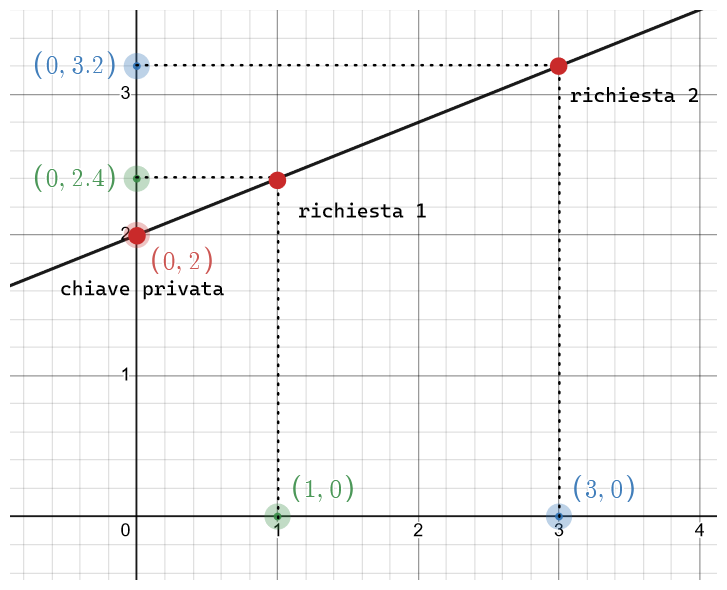
\includegraphics[width=11cm]{./chapters/2.rln-protocol/images/6.a_0_interpolation.png}
    \label{fig:a_0_interpolation}
    \captionsetup{justification=centering}
    \caption{Grafico SSS pilinomio primo grado}
\end{figure}
RLN utilizza l'algoritmo Shamir's Secret Sharing (SSS) che permette di suddividere un segreto in $n$ parti in cui ciascuna parte del segreto non rivela nulla, ma se ne vengono combinate $k$ dove $k < n$ allora il segreto può essere ricostruito. l'algoritmo SSS utilizza l'interpolazione di lagrange per  Per compredere il tutto riportamoci ad un esempio immaginiamo di voler implementare una regola del tipo "Un utente non deve poter effettuare più di 1 richiesta al minuto"
\section{Punizione}
L'ultima fase del protocollo consiste nella punizione dell'utente malintenzionato. Questa procedura è fortemente legata
al contesto applicativo. L'idea generale è che se sono presenti $k$ porzioni diverse per ricostruire
$a_0$ dalle coordinate $x$ e $y$, allora l'identità dell'utente può essere rivelata e l'utente può essere rimosso
dall'albero di Merkle ricostruendo il suo l'identity commitment. Questo comporta
l'azzeramento della foglia che contiene l'identity commitment dell'utente all'interno dell'albero. Inoltre, a seconda dell'applicazione,
la chiave privata può anche essere usata per sequestrare la stake fornita dall'utente.
